%! alt Acute triangle ABC drawn for h = 30, with base BC horizontal. The altitude AD from A to BC has length 20, the altitude BE from B to CA has length 21, and the altitude CF from C to AB is shown. All three feet lie inside their sides and are marked with right angles.
%! after_paragraph 3
%! scale 2/9
% The shared preamble of every Cevian figure. pipeline/figures turns these colours into theme-aware paint,
% and refuses any other colour, so draw only with them:
%   figink (lines and labels), figaux (construction lines), figaccent (the object the argument turns on),
%   figtint and figaccenttint (light fills).
\documentclass[border=1.5pt]{standalone}
\usepackage{tkz-euclide}
\definecolor{figink}{RGB}{0,0,0}
\definecolor{figaux}{RGB}{85,85,85}
\definecolor{figaccent}{RGB}{192,57,43}
\definecolor{figtint}{RGB}{221,221,221}
\definecolor{figaccenttint}{RGB}{245,213,208}
% tkz-euclide's defaults draw circles, compasses and marks in 50% grey and fill points with a tint.
\makeatletter
\def\tkz@otherlinecolor{figink}
\def\tkz@euc@circlecolor{figink}
\def\tkz@euc@compasscolor{figink}
\def\tkz@euc@mkcolor{figink}
\def\tkz@mk@fill{figink}
\def\tkz@euc@pointfillcolor{figink}
\makeatother
\tkzSetUpLine[color=figink,line width=.7pt]
\tkzSetUpArc[color=figink,line width=.7pt]
\tkzSetUpCompass[color=figink,line width=.5pt]
\tkzSetUpPoint[color=figink,fill=figink,size=3.1pt]
\tikzset{
  every picture/.style={line cap=round,line join=round,color=figink},
  circle style/.append style={color=figink,line width=.7pt},
  aux/.style={color=figaux,line width=.45pt,dash pattern=on 2.6pt off 2pt},
  key/.style={color=figaccent,line width=1pt},
  mk/.style={color=figink,line width=.5pt},
  lbl/.style={color=figink,inner sep=2.2pt},
  len/.style={color=figink,inner sep=1.5pt,font=\small},
}

\begin{document}
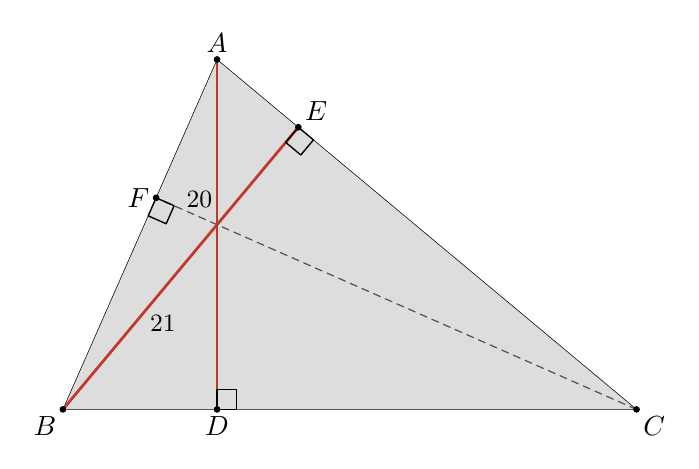
\begin{tikzpicture}
%! let x0 = 1/20
%! let y0 = 1/21
%! let z0 = 1/30
%! let K0 = sqrt(2*(x0**2*y0**2+y0**2*z0**2+z0**2*x0**2) - (x0**4+y0**4+z0**4))/4
%! let k = 1/(2*K0)
%! let a = k*x0
%! let b = k*y0
%! let c = k*z0
\tkzDefPoint(0.0,0.0){B} %! B = (0, 0)
\tkzDefPoint(7.2845971,0.0){C} %! C = (a, 0)
\tkzDefPoint(1.9574257,4.4444444){A} %! A = ((a**2+c**2-b**2)/(2*a), 20)
\tkzDefPoint(1.9574257,0.0){D} %! D = foot(A, B, C)
\tkzDefPoint(2.9895652,3.5833333){E} %! E = foot(B, C, A)
\tkzDefPoint(1.1834436,2.6870748){F} %! F = foot(C, A, B)
%! fact dist(A, D) == 20
%! fact dist(B, E) == 21
%! fact on_segment(D, B, C)
%! fact on_segment(E, C, A)
%! fact on_segment(F, A, B)
%! fact perp(A, D, B, C)
%! fact perp(B, E, C, A)
%! fact perp(C, F, A, B)
\tkzFillPolygon[color=figtint](A,B,C)
\tkzDrawPolygon(A,B,C)
\tkzDrawSegment[key](A,D)
\tkzDrawSegment[key](B,E)
\tkzDrawSegment[aux](C,F)
\tkzMarkRightAngle[size=.25,mk](A,D,C)
\tkzMarkRightAngle[size=.25,mk](B,E,C)
\tkzMarkRightAngle[size=.25,mk](C,F,B)
\tkzDrawPoints(A,B,C,D,E,F)
\tkzLabelPoint[above,lbl](A){$A$}
\tkzLabelPoint[below left,lbl](B){$B$}
\tkzLabelPoint[below right,lbl](C){$C$}
\tkzLabelPoint[below,lbl](D){$D$}
\tkzLabelPoint[above right,lbl](E){$E$}
\tkzLabelPoint[left,lbl](F){$F$}
\tkzLabelSegment[left,pos=.4,len](A,D){$20$}
\tkzLabelSegment[below right,pos=.35,len](B,E){$21$}
\end{tikzpicture}
\end{document}
